\documentclass[notitlepage,letterpaper,fleqn]{report}
\usepackage[margin=1in]{geometry}
\usepackage[utf8]{inputenc}
\usepackage{amsmath}
\usepackage{amssymb}
\usepackage{amsfonts}
\usepackage{graphicx}


\title{Westergaard Solutions For Circular Load Areas}
\author{Prepared by: Dr. Armen Amirkhanian, P.E.}
\date{Last Updated: March 2019}

\begin{document}

\maketitle
The following symbol abbreviations are used in this equation sheet:

\begin{tabular}{cp{0.99\textwidth}}
  $E$ & elastic modulus of the concrete, if no prior knowledge, use 4,000,000 psi \\
  $h$ & thickness of concrete slab \\
  $\nu$ & Poisson ratio of concrete, if no prior knowledge, use 0.15 \\
  $k$ & modulus of subgrade reaction (aka subgrade modulus, "k-value", Winkler spring constant) \\
  $\ell$ & radius of relative stiffness, if insufficient information to calculate, assume 36 inches\\
  $P$ & applied load to circular area\\
  $a$ & radius of circular load area\\
  $\sigma$ & stress at bottom of slab, subscripts $i$, $e$, and $c$ represent interior, edge, and corner, respectively\\
  $\Delta$ & deflection of slab at load, subscripts $i$, $e$, and $c$ represent interior, edge, and corner, respectively
\end{tabular}\\

All of Westergaard's solutions rely on a term called \textit{radius of relative stiffness} \cite{HM1926} shown in Eq. \ref{eq:relative stiffness}. The radius of the loaded area, $a$, is related to the cone of equivalent distribution, $b$, by the relationship shown in Eq. \ref{eq:AB} and described in further detail in \cite{HM1926}. 

\begin{equation}
\ell=\left(\dfrac{Eh^{3}}{12\left(1-\nu^{2}\right)k}\right)^{0.25}
\label{eq:relative stiffness}
\end{equation}

\begin{equation}
\begin{matrix}
b=a & \mathrm{when}  & a\geq 1.724h \\ 
b=\sqrt{1.6a^2+h^2}-0.675h & \mathrm{when}  & a < 1.724h 
\end{matrix}
\label{eq:AB}
\end{equation}

\begin{figure}
    \centering
    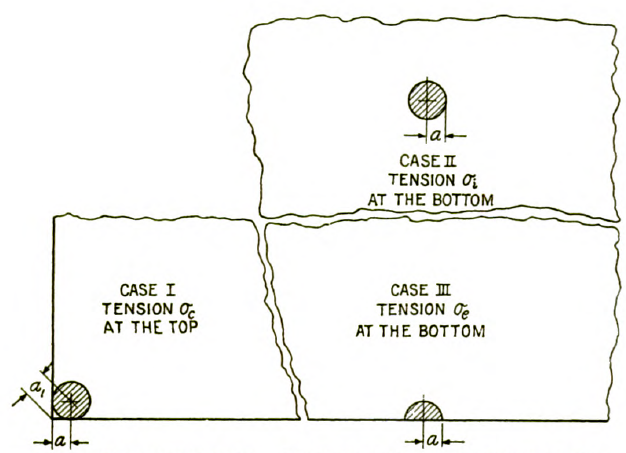
\includegraphics[width=0.4\textwidth]{wes-loading.png}
    \caption{Three specific loading cases solved by Westergaard. From \cite{HM1926}}
    \label{fig:wesload}
\end{figure}

Often times, you are simply provided the wheel load, $P$, and tire pressure, $t_p$, not necessarily the radius of the circular loaded area. However, the radius of the circular area can be calculated via Eq. \ref{eq:tire}.

\begin{equation}
a = \sqrt{\dfrac{P}{\pi t_p}}
\label{eq:tire}
\end{equation}

The calculation of stress and deflection for an infinite slab on a dense liquid foundation (i.e. Winkler foundation) loaded in the interior (Eqs. \ref{eq:cir interior stress} and \ref{eq:cir interior def}), edge (Eqs. \ref{eq:cir edge stre} and \ref{eq:cir edge def}), and corner (Eqs. \ref{eq:cir corner stre} and \ref{eq:cir corner def}) locations are shown below as described in the references \cite{HM1926,HM1939,HM1948,Ioannides1986}.

\begin{equation}
\sigma_{i}=\dfrac{3\left(1+\nu\right)P}{2\pi h^{2}}\left[\ln\left(\dfrac{\ell}{b}\right)+0.6159\right]
\label{eq:cir interior stress}
\end{equation}

\begin{equation}
\Delta_{i}=\dfrac{P}{8k\ell^{2}}\left[1+\dfrac{1}{2\pi}\left(\ln\left(\dfrac{a}{2\ell}\right)-0.673\right)\left(\dfrac{a}{\ell}\right)^{2}\right]
\label{eq:cir interior def}
\end{equation}

\begin{equation}
\sigma_{e}=\dfrac{3\left(1+\nu\right)P}{\pi\left(3+\nu\right)h^{2}}\left[\ln\left(\dfrac{Eh^{3}}{100ka^{4}}\right)+1.84-\dfrac{4\nu}{3}+\dfrac{1-\nu}{2}+\dfrac{1.18\left(1+2\nu\right)a}{\ell}\right]
\label{eq:cir edge stre}
\end{equation}

\begin{equation}
\Delta_{e}=P\sqrt{\dfrac{2+1.2\nu}{Eh^{3}k}}\left(1-\dfrac{\left(0.76+0.4\nu\right)a}{\ell}\right)
\label{eq:cir edge def}
\end{equation}

\begin{equation}
\sigma_{c}=\dfrac{3P}{h^{2}}\left(1-\left(\dfrac{a\sqrt{2}}{\ell}\right)^{0.6}\right)
\label{eq:cir corner stre}
\end{equation}

\begin{equation}
\Delta_{c}=\dfrac{P}{k\ell^{2}}\left(1.1-\dfrac{0.88a\sqrt{2}}{\ell}\right)
\label{eq:cir corner def}
\end{equation}

\vspace{1.5in}

This equation sheet was created from the following primary sources:
\begingroup
\renewcommand{\section}[2]{}%
\renewcommand{\chapter}[2]{}% for other classes
\bibliographystyle{pnas}
\bibliography{Westergaard}
\endgroup

\begin{center}

\includegraphics[scale=0.6]{88x31.png}\\
This equation sheet by Dr. Armen N Amirkhanian is licensed under a Creative Commons Attribution-ShareAlike 4.0 International License.
\end{center}

\end{document}
